\documentclass[conference]{IEEEtran}
% \documentclass{report}

\usepackage{cite}
\usepackage{graphicx}
\usepackage{algorithmic}
\usepackage{amsmath}
\usepackage{amsfonts} % for "\mathbb" macro
\usepackage[caption=false,font=normalsize,labelfont=sf,textfont=sf]{subfig}
\usepackage{url}
\usepackage{hyperref}
\usepackage{float}
\usepackage{listings}
% Customizing lstlisting to mimic verbatim
\lstset{
  basicstyle=\ttfamily,
  breaklines=true, % Allows line breaks
  postbreak=\mbox{\space}, % Optional: mark line breaks
  escapeinside={(@}{@)}, % Define escape characters
}

\newcommand{\N}{\mathbb{N}}
\newcommand{\Z}{\mathbb{Z}}
\newcommand{\Q}{\mathbb{Q}}
\newcommand{\R}{\mathbb{R}}
\newcommand{\C}{\mathbb{C}}


\begin{document}
\title{Phisical Layer Security using Reconfigurable Intelligent Surfaces in Multiple Users and Multiple Reflections MIMO Communications}


% author names and affiliations
% use a multiple column layout for up to three different
% affiliations
\author{
  \IEEEauthorblockN{Simone Marrocco - 239951}
  \IEEEauthorblockA{simone.marrocco@studenti.unitn.it}
}

% make the title area
\maketitle

% As a general rule, do not put math, special symbols or citations in the abstract
% \begin{abstract}
%   TODO
% \end{abstract}


% For peerreview papers, this IEEEtran command inserts a page break and creates the second title. It will be ignored for other modes.
\IEEEpeerreviewmaketitle

\section{Introduction}
\subsection{Physical Layer Security}

Modern technologies, like the Internet of Things (IOT) and the Cooperative Autonomous Driving (CAV), are becoming more and more popular and necessary in our society. However, they also bring new security concerns, especially in the wireless communications.

We have two type of threats we need to protect against. Active attacks, like jamming a frequency, distrupt and block the flow of information; while passive attacks, like eavesdropping, are more subtle and we need to make our signals undeciphrable with encryption or noise. There are different methods we can use to mask our communications: we can fingerprint the legitimate users, spread it through multiple frequencies, use directional antennas or artificial noise schemes \cite{5751298}.

The adversaries may also have better resources, both in computer power and signal reception, and it is difficult to model all possible threats we may face \cite{7120011}.

In particular to eavesdropping, there is a huge opportunity for improvements. While distruptions have been studied for long, especially in military communications, message encryption is usually delegated to the higher levels \cite{6739367}. However, the physical layer can assist by hiding or masking the signal, making it harder for the eavesdropper to capture the it. Given the advances in quantum computing and encryption breaking \cite{365700}, it is important to be protected at all layers.

Achieving perfect communication secrecy is not really possible for all cases, given that we need the secret key to be at least as big as the secret message \cite{6769090}, but there are some practical strategies we can implement.

In \cite{7543509} a statistical model is created to calculate the probability of achieving secrecy from eavesdroppers in unknown locations, while in \cite{4543070} and \cite{1605889} it is discussed how we can use the antenna spare power to induce artificial noise to assure the legitimate receiver has better signal.

\subsection{Reconfigurable Intelligent Surface}

Reconfigurable Intelligent Surfaces (RISs) are a new technology that can help in improving the security of wireless communications. They are made of a large number of passive elements that can reflect the signals in a way that can be controlled and optimized.

With RISs, it is possible to control the propagation and reflection of signals, making it possible to transform the environment, in which the waves need to travel, from an uncontrollable phenomena to a programmable variable that is possible to (partially) control and optimize \cite{9086766}.

RISs can help in particular in two scenarios. In the first one, two nodes which are not in the line of sight (LOS) can communicate with the help of the RIS; in the second one, being in the LOS means an inability to take advantage of delayed reflections (especially for new technologies like 5G and 6G), which can be used to improve the signal quality and robustness, but we can create them with RISs \cite{9086766}.

The main advantages of RISs are the low cost, the low power consumption and the easy deployment, which makes them a good candidate for the future of wireless communications. They do not require a dedicated energy source, they do not suffer from noise amplification, they can work with any frequency and can be easly put in any surface like walls or ceilings \cite{8796365}.

\subsection{Using RISs for Physical Layer Security}

RISs can be used to greatly increase not only the network performance but also its security \cite{10409564}. By using RISs, we can make the signal quality better, reduce the signal degradation and make the signal more difficult to intercept by eavesdroppers.

For example, the reflection can be used as multiplicative randomness to make the transmission not understable from eavesdroppers, while having a decoding for the legitimate user linear \cite{9328149}.

Another paper \cite{s21041439} studied how to use a novel RIS based channel randomization technique to improve the secrecy rate, and another one \cite{8742603} shows an iterative efficient algorithm to maximize the minimum secrecy rate by optimizing the reflecting coefficients of the RIS.

RISs can also be used to protect against jamming attacks: for example, in \cite{9424472} it is used an aerial RIS to mitigate the effects of the disturbance and increase the transmission power and reliability.

\subsection{RISs and Physical Layer Security for Vehicular Networks}

Cooperative autonomous driving can bring many benefits, like reducing traffic congestion, improving road safety and reducing the environmental impact of the vehicles. Cars and other vehicles can communicate with each other and with the infrastructure to share information and coordinate their movements. However, it also brings new security concerns, especially in the wireless communications.

It is clear that it is necessary to have a secure and fast way to communicate, and 6G network technologies plus RISs can help in this regard. By reflecting the signals, we can overcome the limitations of LOS and improve the signal quality by reducing signal degradation \cite{10715713}.

The sector is just starting to be studied, but there are already some promising result. Network simulators made specific, like CoopeRIS, allow to study and progress this field \cite{SEGATA2024110443}.

Vehicular networks need low latency and high security. Active attack may jeopardize drivers' and people's safety, while also slowing down information exchange rate. Being moving agents, it is more difficult to correctly model this type of network, but also way more necessary: complex upper layer encryption may slow down data processing enough to render it useless \cite{8403278}.

Passive attackers may instead use vehicles' geolocation and traffic data for malicious activity. A way to detect and filter out intruders is discussed in \cite{8474336}.

Recent studies shows how RISs can be used to protect the vehicular network against illegitimate users. In \cite{makarfi2020reconfigurableintelligentsurfacesenabledvehicular} the authors study how RISs can improve the average secrecy capacity and secrecy outrage probability.

\subsection{Future Directions}

Network intensive technologies like IOT and CAV are gaining traction fast, thanks to the many benefits they bring to society and the newest technologies that now allow this incredibly huge traffic load.

However, the security of these networks is still a big concern, and it is necessary to study and implement new technologies to protect them. RISs are a promising technology that can help in this regard. Being cost effective, fairly passive and easy to deploy, they can assist in overcoming the problems of 6G like signal fading and out of LOS communication \cite{8796365}.

However, while we have some initial literature in both physical layer security using RISs, and using RISs to improve vehicular network performances, not much has been made in studying all three of these aspects \cite{makarfi2020reconfigurableintelligentsurfacesenabledvehicular}.

Practical solutions could be studied and simulated starting from the resources presented here. RISs can be used both to mask the network signal or to make it noisier for unwanted listeners located in different places.

For example, starting from \cite{4543070}, it could be studied how cooperating vehicles could calculate together with a RIS how to add noise to other locations while moving in space, and so needing constant modifications in the calculations themselves.

Modern cars have as much computing power as a modern personal computer: for example, Tesla cars have an integrated GPU to utilize the autonomus driving feature \cite{10586734}, which could be used for highly efficient matrix calculations \cite{1011452699470}.

In conclusion, the future of vehicular networks is bright, but it is necessary to study and implement new technologies to protect them. RISs are a promising technology that can help in this regard, and it is necessary to study how to use them to improve the security of vehicular networks.
\section{Hidden comunication by targeted reflections}

We will start from the paper \textit{Reconfigurable Intelligent Surface: Reflection Design Against Passive Eavesdropping} \cite{9328149}, explaining how to hide communication between two actors from eavesdroppers using Reconfigurable Intelligent Surfaces, then expanding it to multiple receiving users at the same time.

\begin{figure}[H]
  \centering
  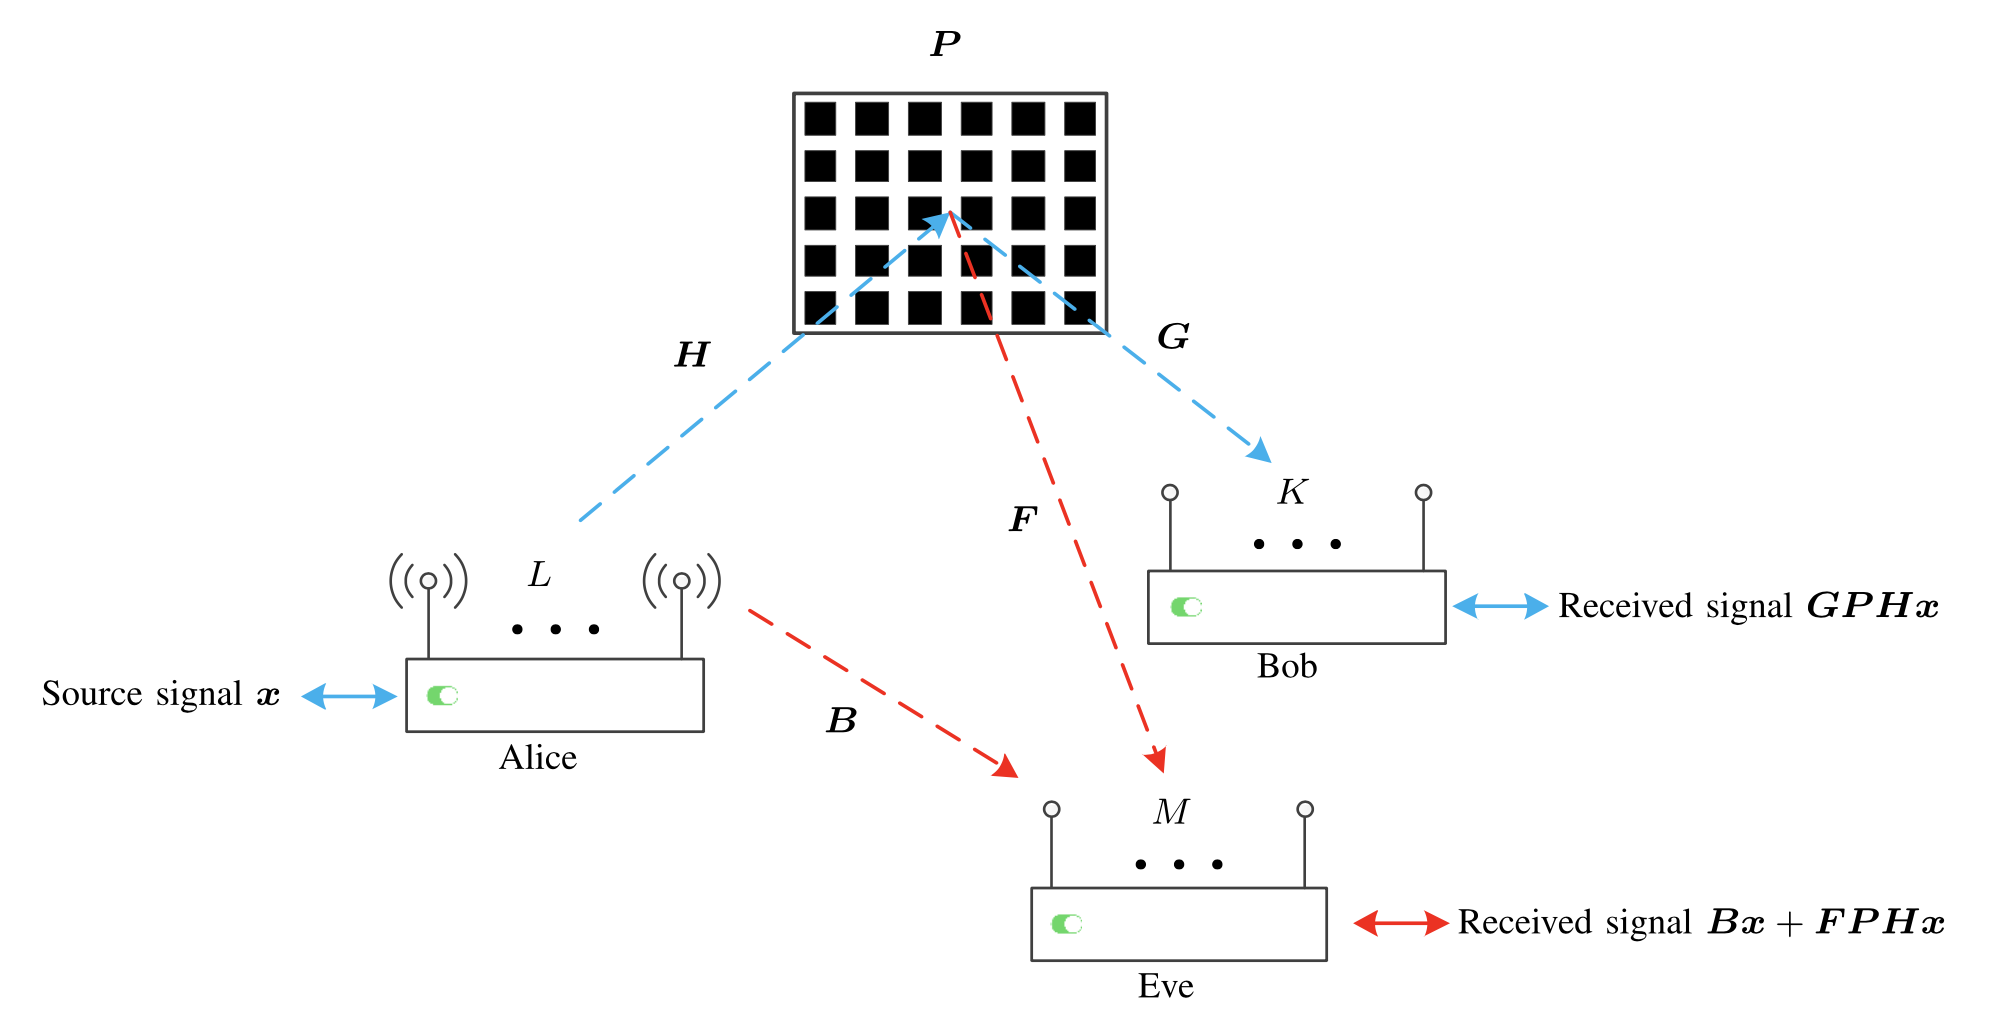
\includegraphics[width=\linewidth]{imgs/problem-description.png}
  \caption{Setup}
  \label{fig:correlation_sk}
\end{figure}

In \cite{9328149}, the authors studied how to use RISs to allow communications between two users without LOS, while making the signal undeciphrable for eavesdroppers. We call $L$ the transmitter's antennas, $K$ the receiver's antennas, $M$ the eavesdropper's antenna, and $N$ the RIS reflecting elements. We assume $L \ge K \ge 2$.

We define $H \in \C^{NxL}$ the channel response from the transmitter to the RIS, $G \in \C^{KxN}$ the channel response from the RIS to the receiver, $P = diag\{p\} \in \C^{NxN}$ a diagonal matrix in which the $n$th diagonal element represents the reflection coefficient of the $n$th unit at the RIS.

The objective is making the receiver's final signal $GPH$ a diagonal matrix, while making every possible eavesdropper's final signal a full matrix.

We will leave for now the technical details of why this would achieve secrecy for the legitimate users to the original paper, and will just focus on the mathematics behind the calculation. It is possible to read more in the paper \textit{Space shift keying modulation for MIMO channels} \cite{5165332}.

Our final objective will be to generalize these calculations to $J$ receving users and multiple RISs used in parallel and in sequence.

Formally, the condition we want to satisfy is:

\begin{equation}
  || [GPH]_{:,1:K} - [[GPH]_{:,1:K}]_{diag} || ^2 = 0
\end{equation}

Where $[GPH]_{:,1:K} \in \C^{KxK}$ denotes the first K columns of the matrix $GPH \in \C^{KxL}$.

Given

\begin{equation}
  W = \sum_{i,j = 1, i \ne j}^{K} (g_{j,:} \odot h_i^T)^H (g_{j,:} \odot h_i^T)
\end{equation}
\begin{equation}
  rank(W) = K(K-1), rank(W) - nullity(W) = N
\end{equation}
\begin{equation}
  nullity(W) = N - (K^2 - K)
\end{equation}

The formula (1) can be rewritten as

\begin{equation}Wp = 0\end{equation}

and the solutions of $p$ can be found in the null space of $W$. Using singular value decomposition (SVD), we can decompose

\begin{equation}
  W = R \Sigma V^H \footnote{An hermitian transpose of $V$ ($V^H$), means we fist transpose the matrix ($V \rightarrow V^T$), then take the conjugate of every element (so invert the sign of the immaginary part).}
\end{equation}

With SVD, we have $\Sigma = diag(\sigma) \in C^{NxN}$ a diagonal matrix. the first $rank(W) = K^2-K$ elements of $\sigma$ are non-zero, while the last $nullity(W) = N - (K^2-K)$ elements are zero. \footnote{\url{https://math.stackexchange.com/questions/1771013/how-is-the-null-space-related-to-singular-value-decomposition}}

Given a more generic $A \in \C^{mxn} = R' \Sigma' V'^H$, we have the column vectors of $R'$ being an orthonormal span of $C^m$, and the row vectors of $V'$ being an orthonormal span of $C^n$.

Suppose $A$ is an Hermitian matrix (meaning $A = A^H$). This will be useful later, as $W$ is also an Hermitian matrix by construction. Let's call $k$ the null space dimension of $A$, and ,by the property above, the null space dimension of $A^H$ too.

The last $k$ columns of $R'$ are a span of the null space
\begin{equation}
  N(A^H) = [r_{m-k}, ..., r_m ] \in \C^{mxk}
\end{equation}
while the last $k$ rows of $V'^H$ are a span of the null space
\begin{equation}
  N(A) = \begin{bmatrix} v'^H_{n-k} \\ ... \\ v'^H_n \end{bmatrix} \in \C^{kxn}
\end{equation}
Being $A$ an Hermitian matrix, the two null spaces are both solutions to $Ax = 0$.

Consider now $W \in C^{NxN}$. The paper in question uses equation (7) to find the solutions, since $W$ is hermitian and square. Taken $U \in \C ^ {Nx(N-(K^2 - K))}$ the last $N-(K^2 - K)$ columns of the left singular matrix $R$. $U \in N(W)$ for the explanation above. We then have

\begin{equation}WU = 0\end{equation}
\begin{equation}p = Uq\end{equation}
\begin{equation}WUq = 0\end{equation}

being true, and $q \in \C^{N-(K^2 - K)}$ can be a random vector.

\section{Expanding to multiple users}

In real life scenarios, we deal with more than two communicating actors. We want to expand the findings of this paper by having it support multiple RISs in series and multiple receivers from the same transmitter. Once we have those, we can generalize it to also have receivers getting signals from multiple indipendent reflections of RISs.

We will first, however, make some semplifications about the actors by having $L = K$ for all of them. We will still consider one transmitter, with $J \ge 1$ receivers.

\subsection{Reflecting to multiple users}

We consider the case where the transmitter wants to send the signal to $J$ receivers without LOS. The condition we want to satisfy is

\begin{equation}
  \forall j \in [1...J] \rightarrow || G_jPH - [G_jPH]_{diag} || ^2 = 0
\end{equation}

\begin{equation}
  \forall j \in [1...J] \rightarrow W_jp = 0
\end{equation}

\begin{equation}
  \begin{bmatrix}
    W_1  \\
    W_ 2 \\
    ...  \\\
    W_j
  \end{bmatrix}
  p = 0
\end{equation}

\begin{equation}
  \begin{bmatrix}
    W_1  \\
    W_ 2 \\
    ...  \\\
    W_j
  \end{bmatrix}
  = W \in \C ^ {JNxN}, W = R \Sigma V^H
\end{equation}

The problem we have now is that $W$ is not a square matrix anymore, so we cannot use the last $N - (K^2 - K)$ columns of $R$ to calculate the null space and $p$ with its linear combination. The null space would have dimension $N(W) \in \C^{JN x (N - (K^2 - K))}$, but we need $p \in C^N$.

We can, however, use the the last $N - (K^2 - K)$ rows of $V^H$, then apply again the hermitian transposition to get our desired solution. Remember that $N(W)$ can also be calculated using the left singular matrix. Since now $W$ is not a square matrix, so $W \ne W^H$,

\begin{equation}
  N(W) = \begin{bmatrix} v^H_{N - J(K^2 - K)} \\ ... \\ v^H_N \end{bmatrix} ^ H
\end{equation}

Take $U_1 \in \C ^ {N - J(K^2 - K) x N}$ the last $N - (K^2 - K)$ rows of $V^H$, and
\begin{equation}
  U = U_1^H \in \C ^ {N x N - J(K^2 - K)}
\end{equation}

We now can apply the same method as before

\begin{equation}p = Uq\end{equation}

\begin{equation}WU = 0\end{equation}

\begin{equation}WUq = 0\end{equation}

\subsection{RISs in parallel}

Given the previous property, it follows that we can use $M$ multiple RIS, each one reflecting the signal to $J$ multiple receivers. For the receiver $j \in [1, J]$, we have

\begin{equation}
  \sum_{m=1}^M G_j P_m H_m x = (\sum_{m=1}^M G_j P_m H_m) x =
\end{equation}

The sum of diagonal matrixes is still a diagonal matrix, so the property still holds.

\subsection{RISs in series}

We consider the case where the signal is bounced between $M$ RISs in this way:

\begin{equation}
  \text{Transmitter} \rightarrow \text{RIS 1} \rightarrow ... \rightarrow \text{RIS M} \rightarrow \text{Receiver}
\end{equation}

We call $C_i \in \C^{NxN}$ the channel gain between $P_i$ and $P_{i+1}$. We need to solve

\begin{equation}
  || GP_1C_1...P_MH - [GP_1C_1...P_MH]_{diag} || ^2 = 0
\end{equation}

We can generate $p_1, ..., p_{M-1}$ as random reflections, and calculate the last one based on the previous. An advantage we get is that eavesdroppers listening from a middle RIS will not be able to decipher the signal either. Given $r_i \in [0, 1]$ the absorption coefficient, and $\theta_i \in [0, 2\pi]$ the phase shift, we can choose them randomly for all RIS $p_m$ vectors, but the last one.

\begin{equation}
  \forall m \in [1, M-1] : p_m[i] = \eta * r_i * e^{j\theta_i}
\end{equation}

Given now

\begin{equation}
  G' = GP_1C_1...P_{M-1}C_{M-1} \in \C^{KxN}
\end{equation}

We can consider now the problem of solving

\begin{equation}
  || G'P_MH - [G'P_MH]_{diag} || ^2 = 0
\end{equation}

Which can be solved as before.
\footnote{It is also possible to set up randomly the last $M-1$ RIS and calculate the first one using $G$ and $H'=C_1P_2C_2...P_M$. The properties still holds.}
\footnote{Estimate the channel gains $G$ and $H$, based on \cite{8879620}, could be more difficult, given that we do not have full controll on $P=P_1C_1...P_M$ anymore. We can however estimate directly $G'$ by keeping the same random $P_1, ..., P_{M-1}$ in both the acknowlegdment round and the message trasmission round, and just modify $P_M$ after estimating $G'$ and $H$ to correctly deliver the message.}

If we have multiple $G_j$, it will be enough to calculate all the $G'_j$ and proceed as before, allowing us to combine these properties in more complicated scenarios.

\section{Simulation Results}

We can now test more complex setups by doing Bit Error Rate (BER) analysis.

\begin{figure}[H]
  \centering
  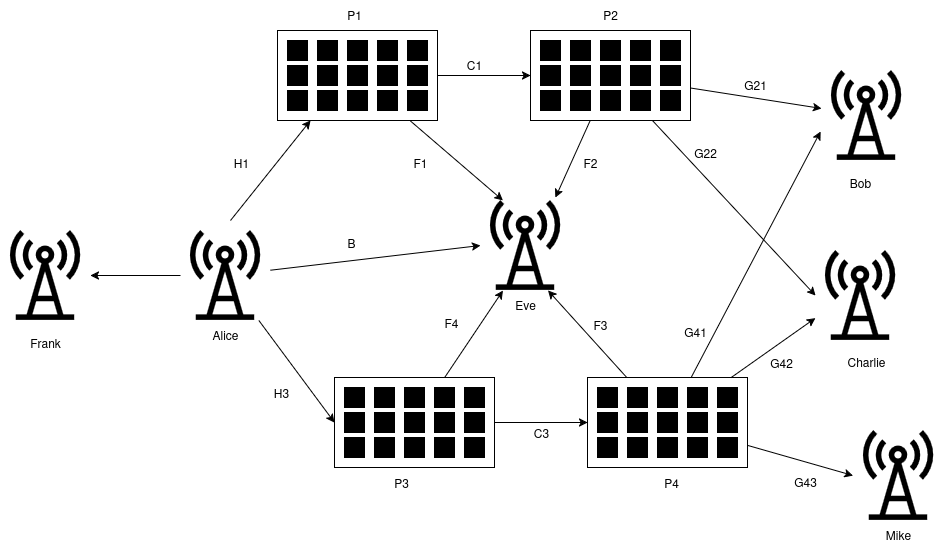
\includegraphics[width=\linewidth]{imgs/complex-situation.png}
  \caption{Complex Setup}
  \label{fig:correlation_sk2}
\end{figure}

For example, here we have a single transmitter \textit{Alice} and multiple receivers. \textit{Frank} is a direct receiver in line of sight. \textit{Bob} and \textit{Charlie} receive the signal from two double RIS reflection. \textit{Eve} receives both the direct signal and the reflecting signal from all RISs. \footnote{It should be noted that if \textit{Eve} is in the same position as \textit{Frank} and receives just the direct signal, our particular framework would not give us physical layer security, and higher layer security would be needed. If instead \textit{Eve} has not line of sight, the message would be completely unreadable from the start, since it would receive random matrixes.}

More in general, we would have $M$ consecutive RIS (in series) that reflect a signal, $J$ legitimate receivers and $Q$ different paths of RIS (in parallel) to send the signal at the same time. \footnote{The paths could have a different number of RIS (for example, a path of three and another of two). The results would still hold.}

We will show simulation results for different combinations of ($M, J$), both with a single and double path. In all scenarios, $K = 2, N = 16, \eta = 0.9$ will be the number of antennas for all actors, the number of reflecting surfaces and the reflection coefficients.

The direct link and the eavesdropper will try to understand the message by following the instructions on \cite{5165332}, while the receivers will try to understand it by following the instructions on \cite{9328149}.

\subsection{Single RIS reflection (M=1)}

\begin{figure}[H]
  \centering
  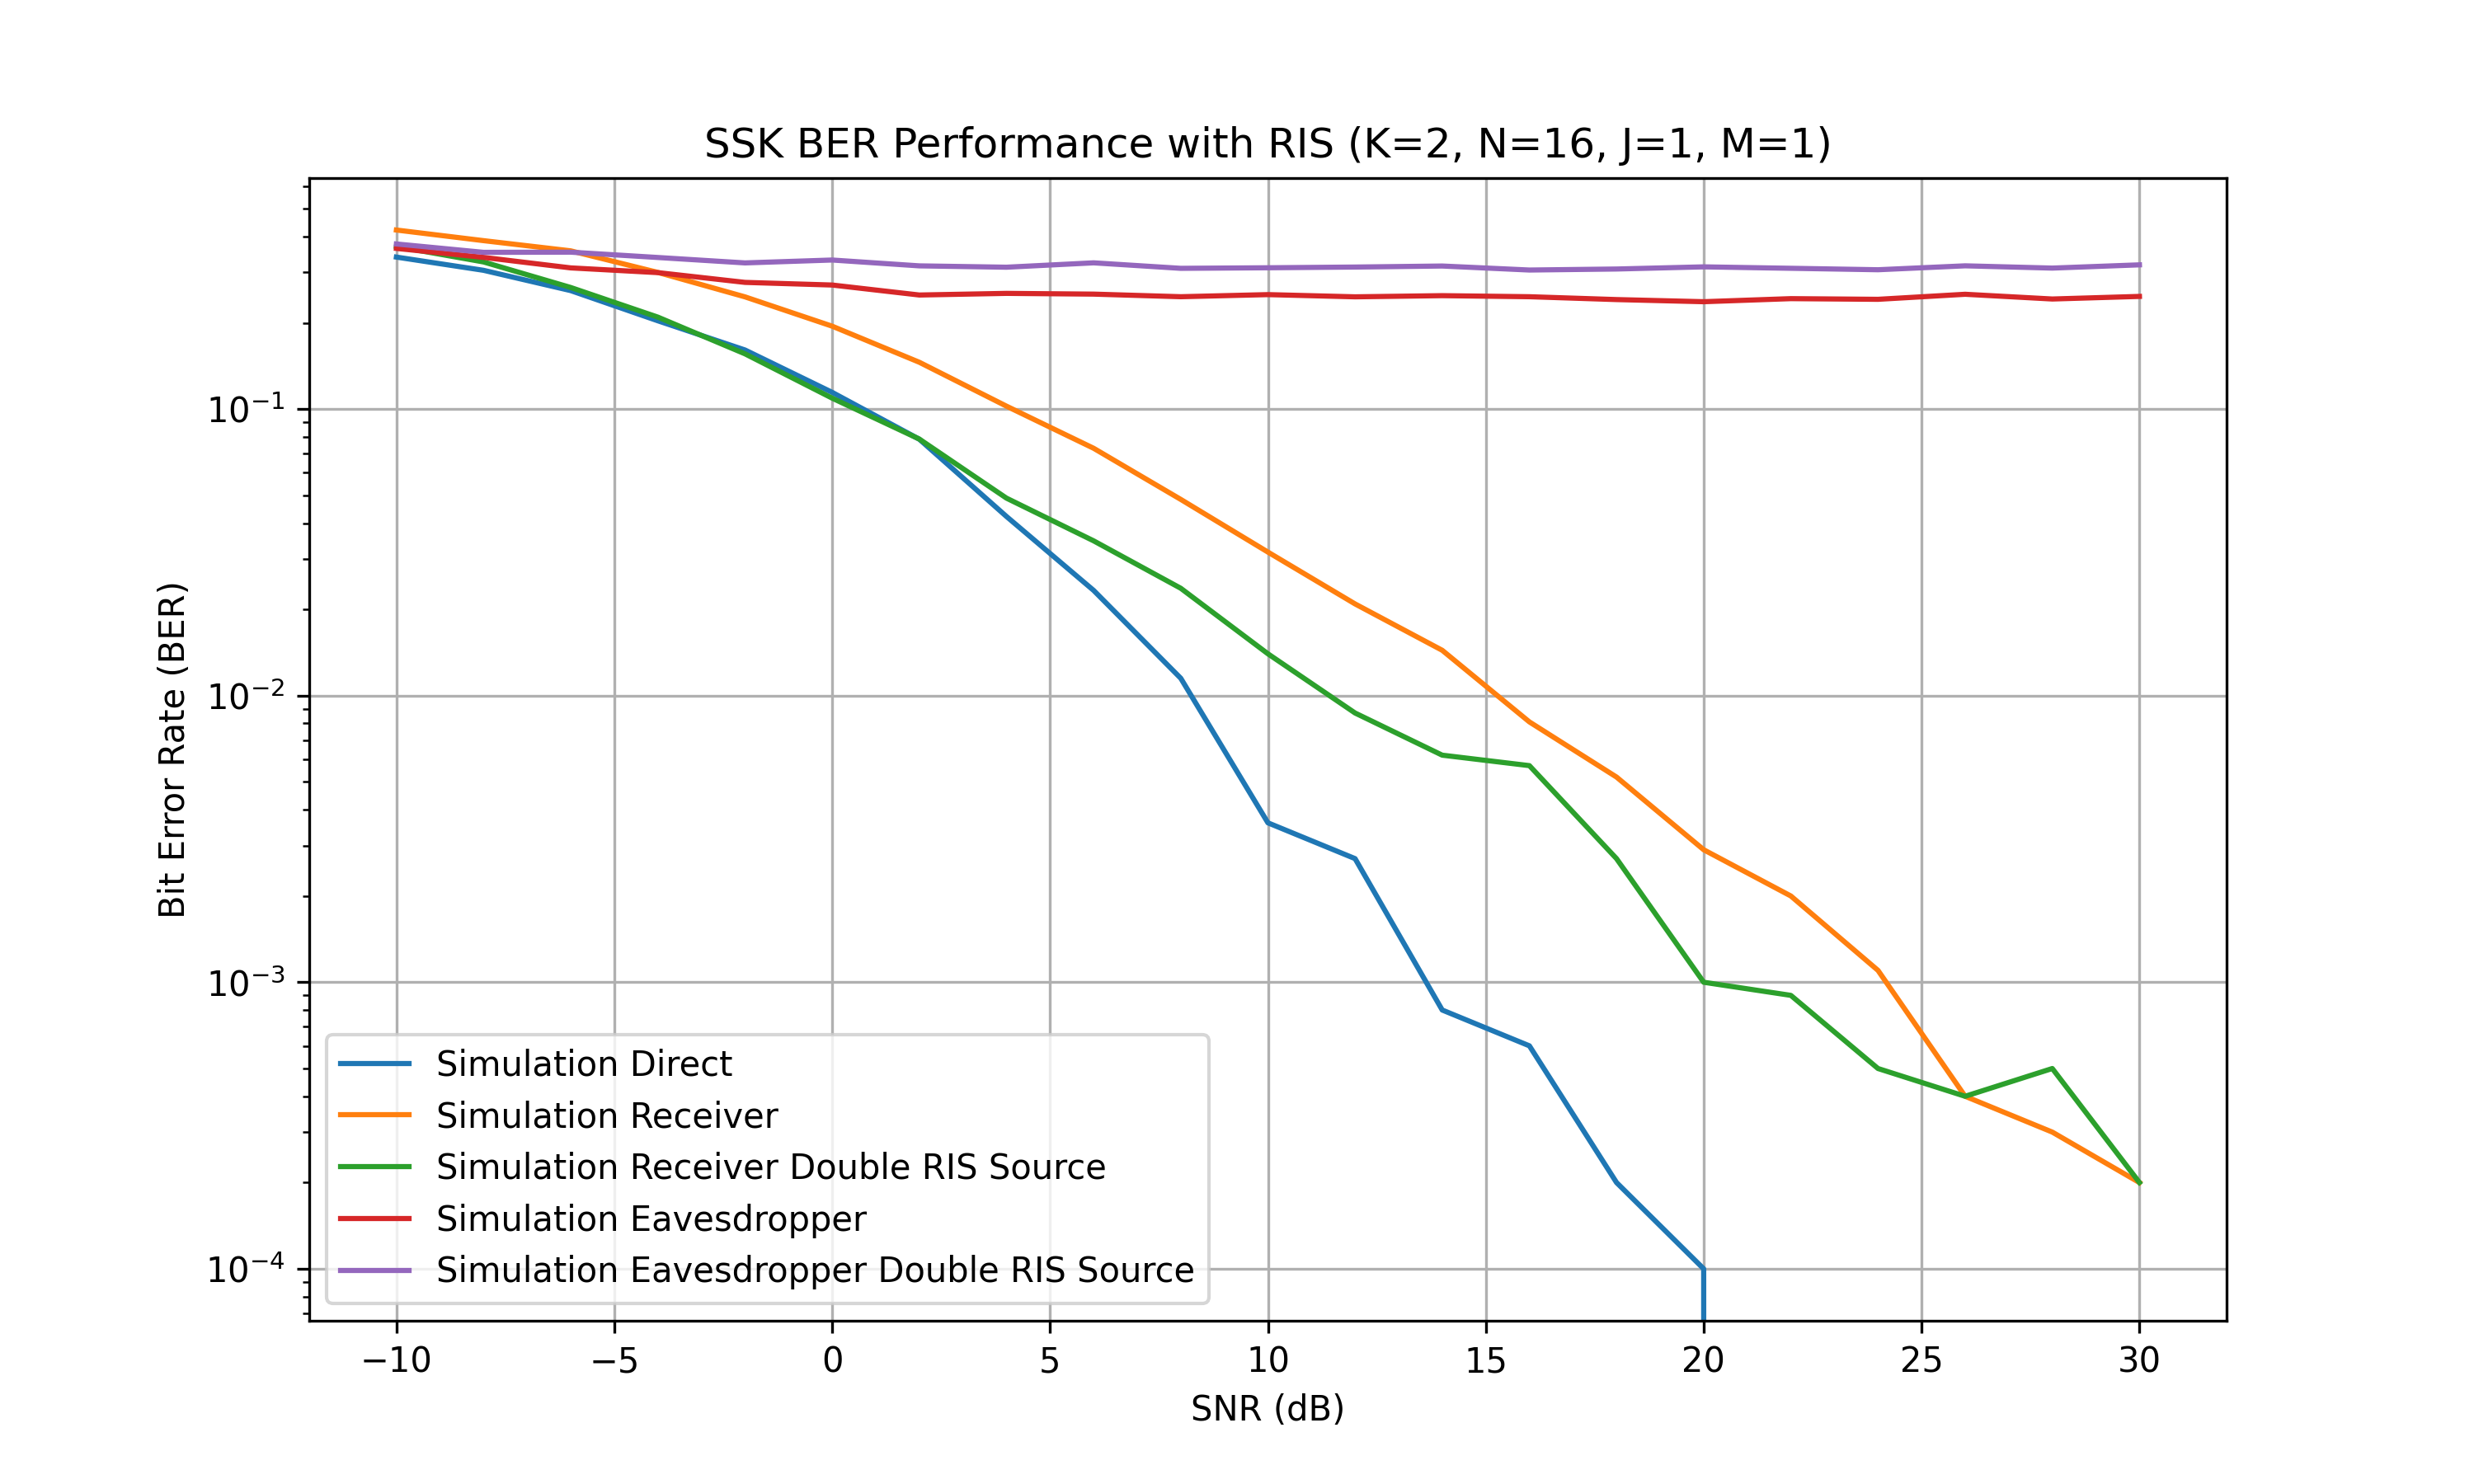
\includegraphics[width=\linewidth]{imgs/ber-simulations/SSK BER Performance with RIS (K=2, N=16, J=1, M=1).png}
  \caption{SSK BER Performance with RIS (K=2, N=16, J=1, M=1)}
  \label{fig:simulation_j1_m1}
\end{figure}

We can see in ($M=1, J=1$) the results match with \cite{9328149}, for both \textit{Simulation Receiver} and \textit{Simulation Eavesdropper}.
\textit{Simulation Direct} is the strongest possible path, mainly because of the reflection loss due to $\eta$.
Combining two different RIS in parallel (\textit{Double RIS Source}) gives better signal to the receiver, while disturbing more the signal to the eavesdropper.

\begin{figure}[H]
  \centering
  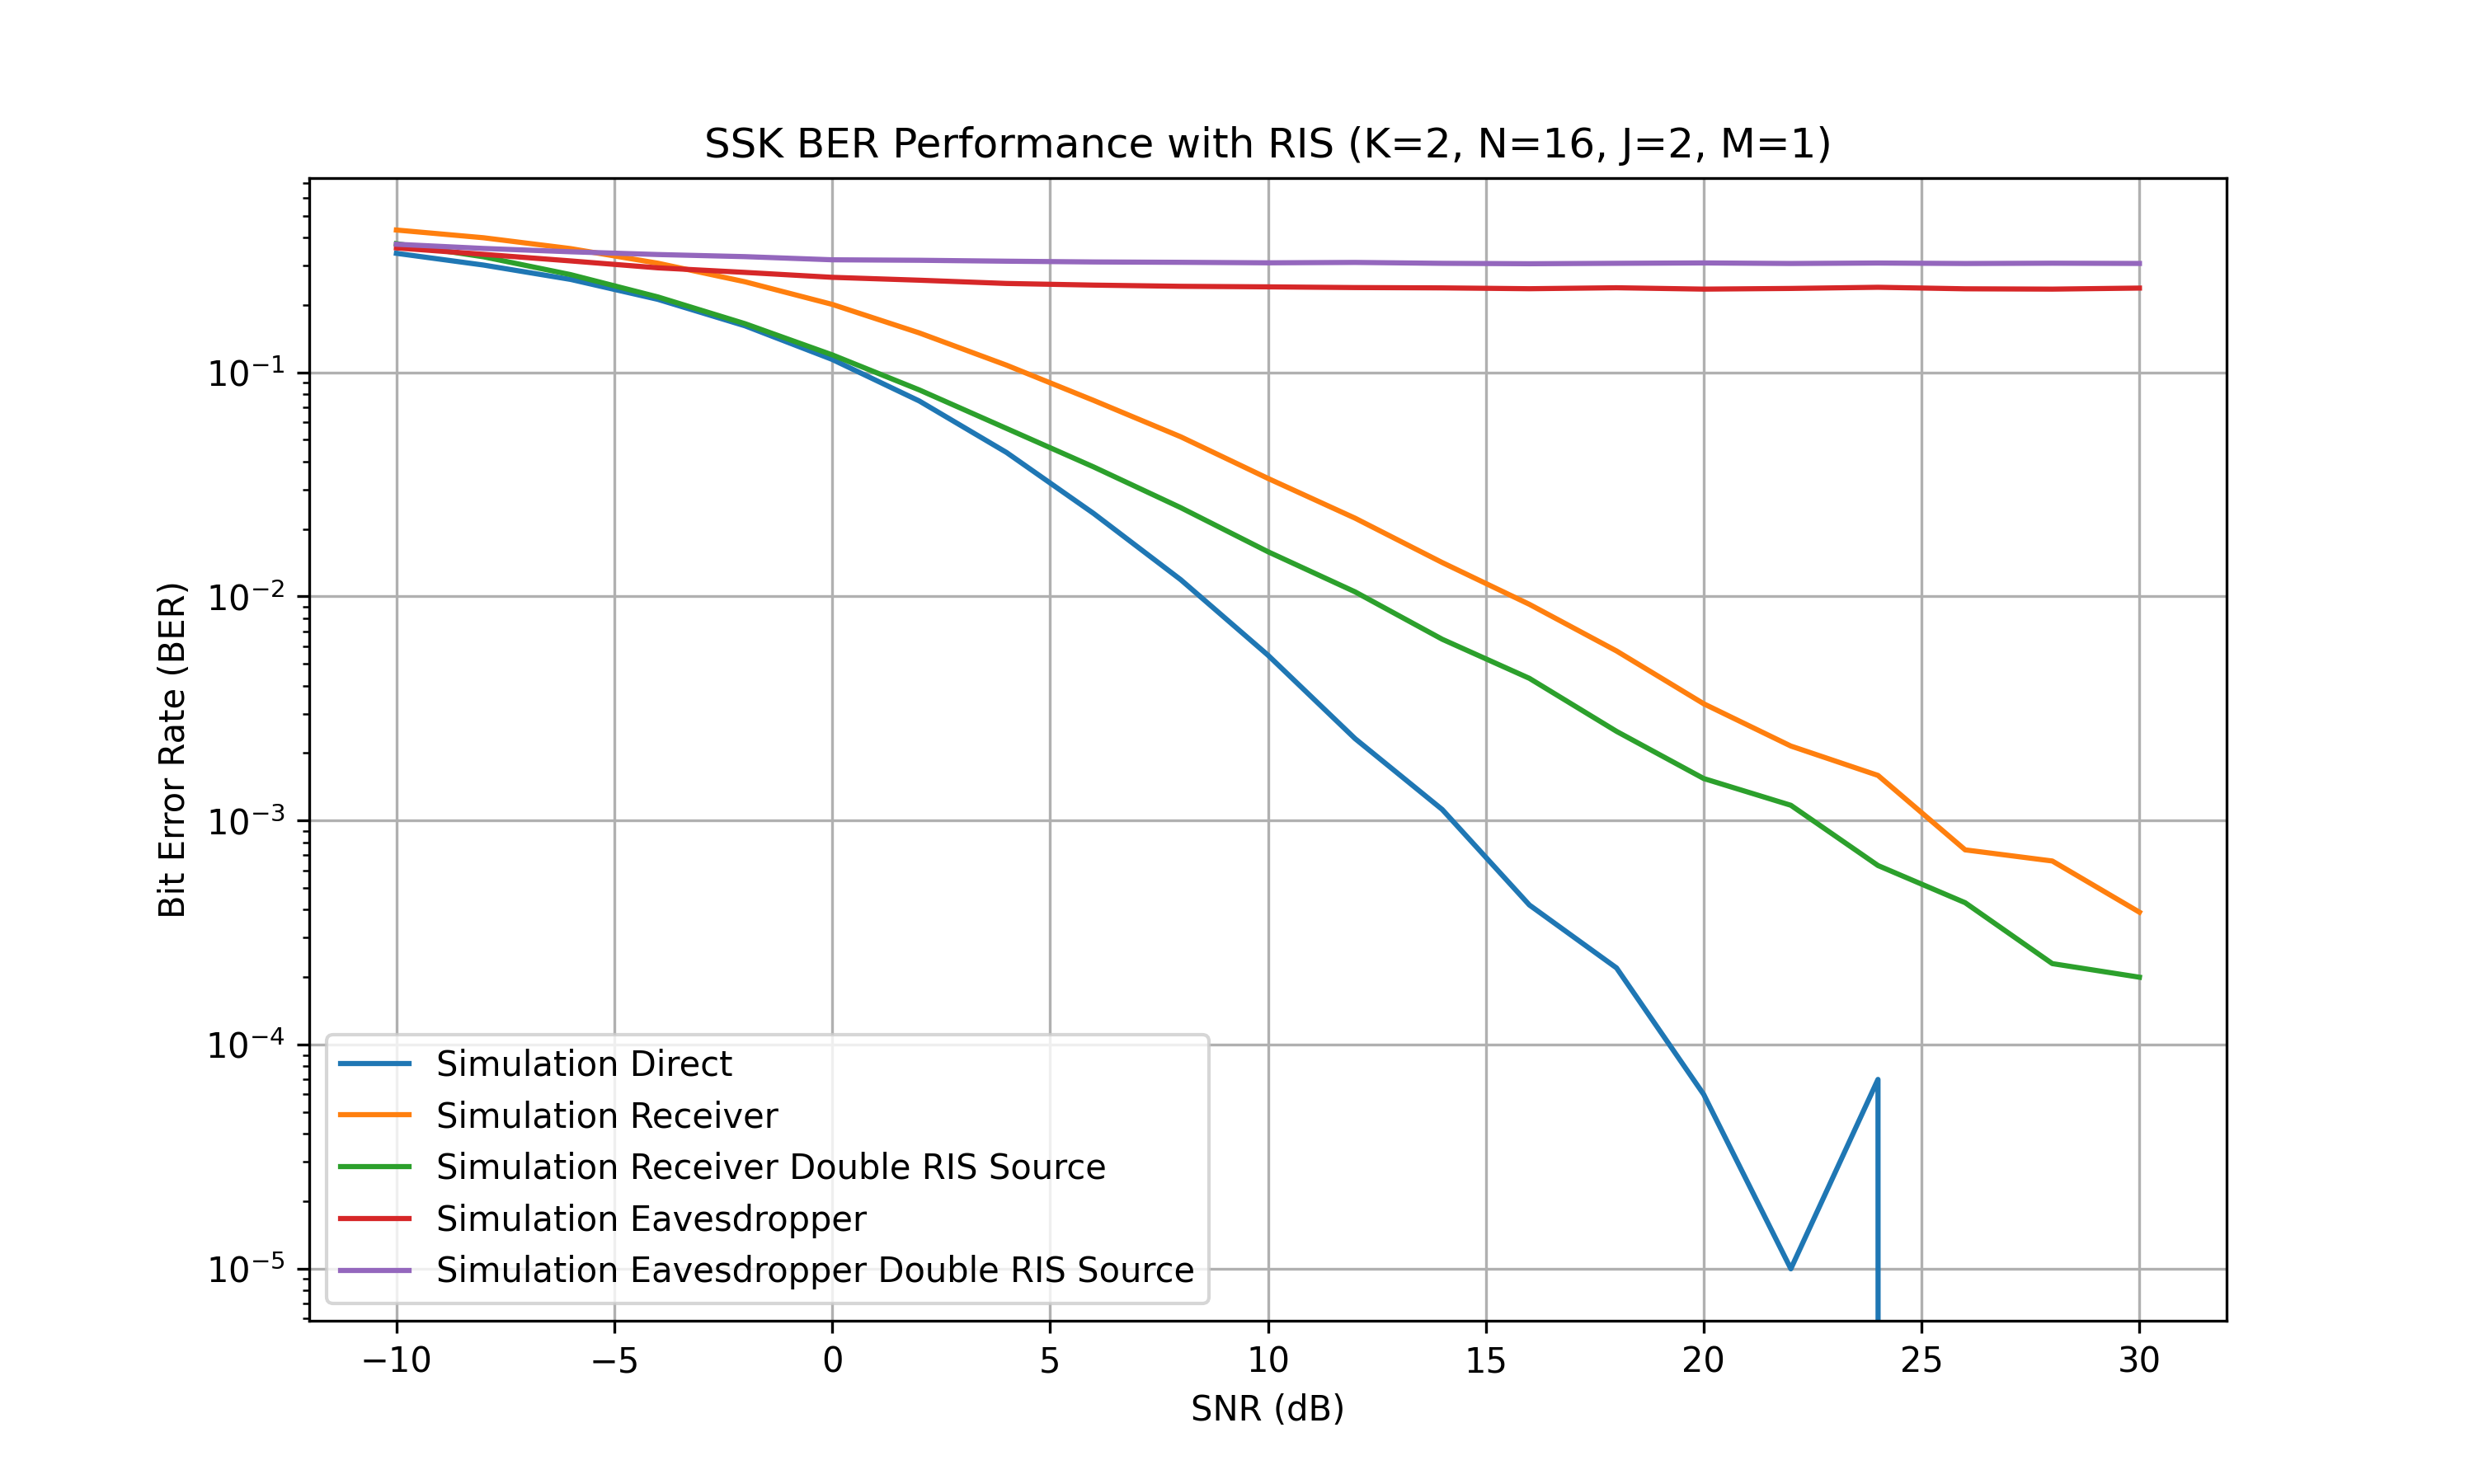
\includegraphics[width=\linewidth]{imgs/ber-simulations/SSK BER Performance with RIS (K=2, N=16, J=2, M=1).png}
  \caption{SSK BER Performance with RIS (K=2, N=16, J=2, M=1)}
  \label{fig:simulation_j2_m1}
\end{figure}

Increasing the number of receivers does not influence the result of our framework: the receivers still get a good signal depending on the SNR, while the eavesdropper is not getting an advantage in understanding the message.

\subsection{Double RIS reflection (M=2)}

\begin{figure}[H]
  \centering
  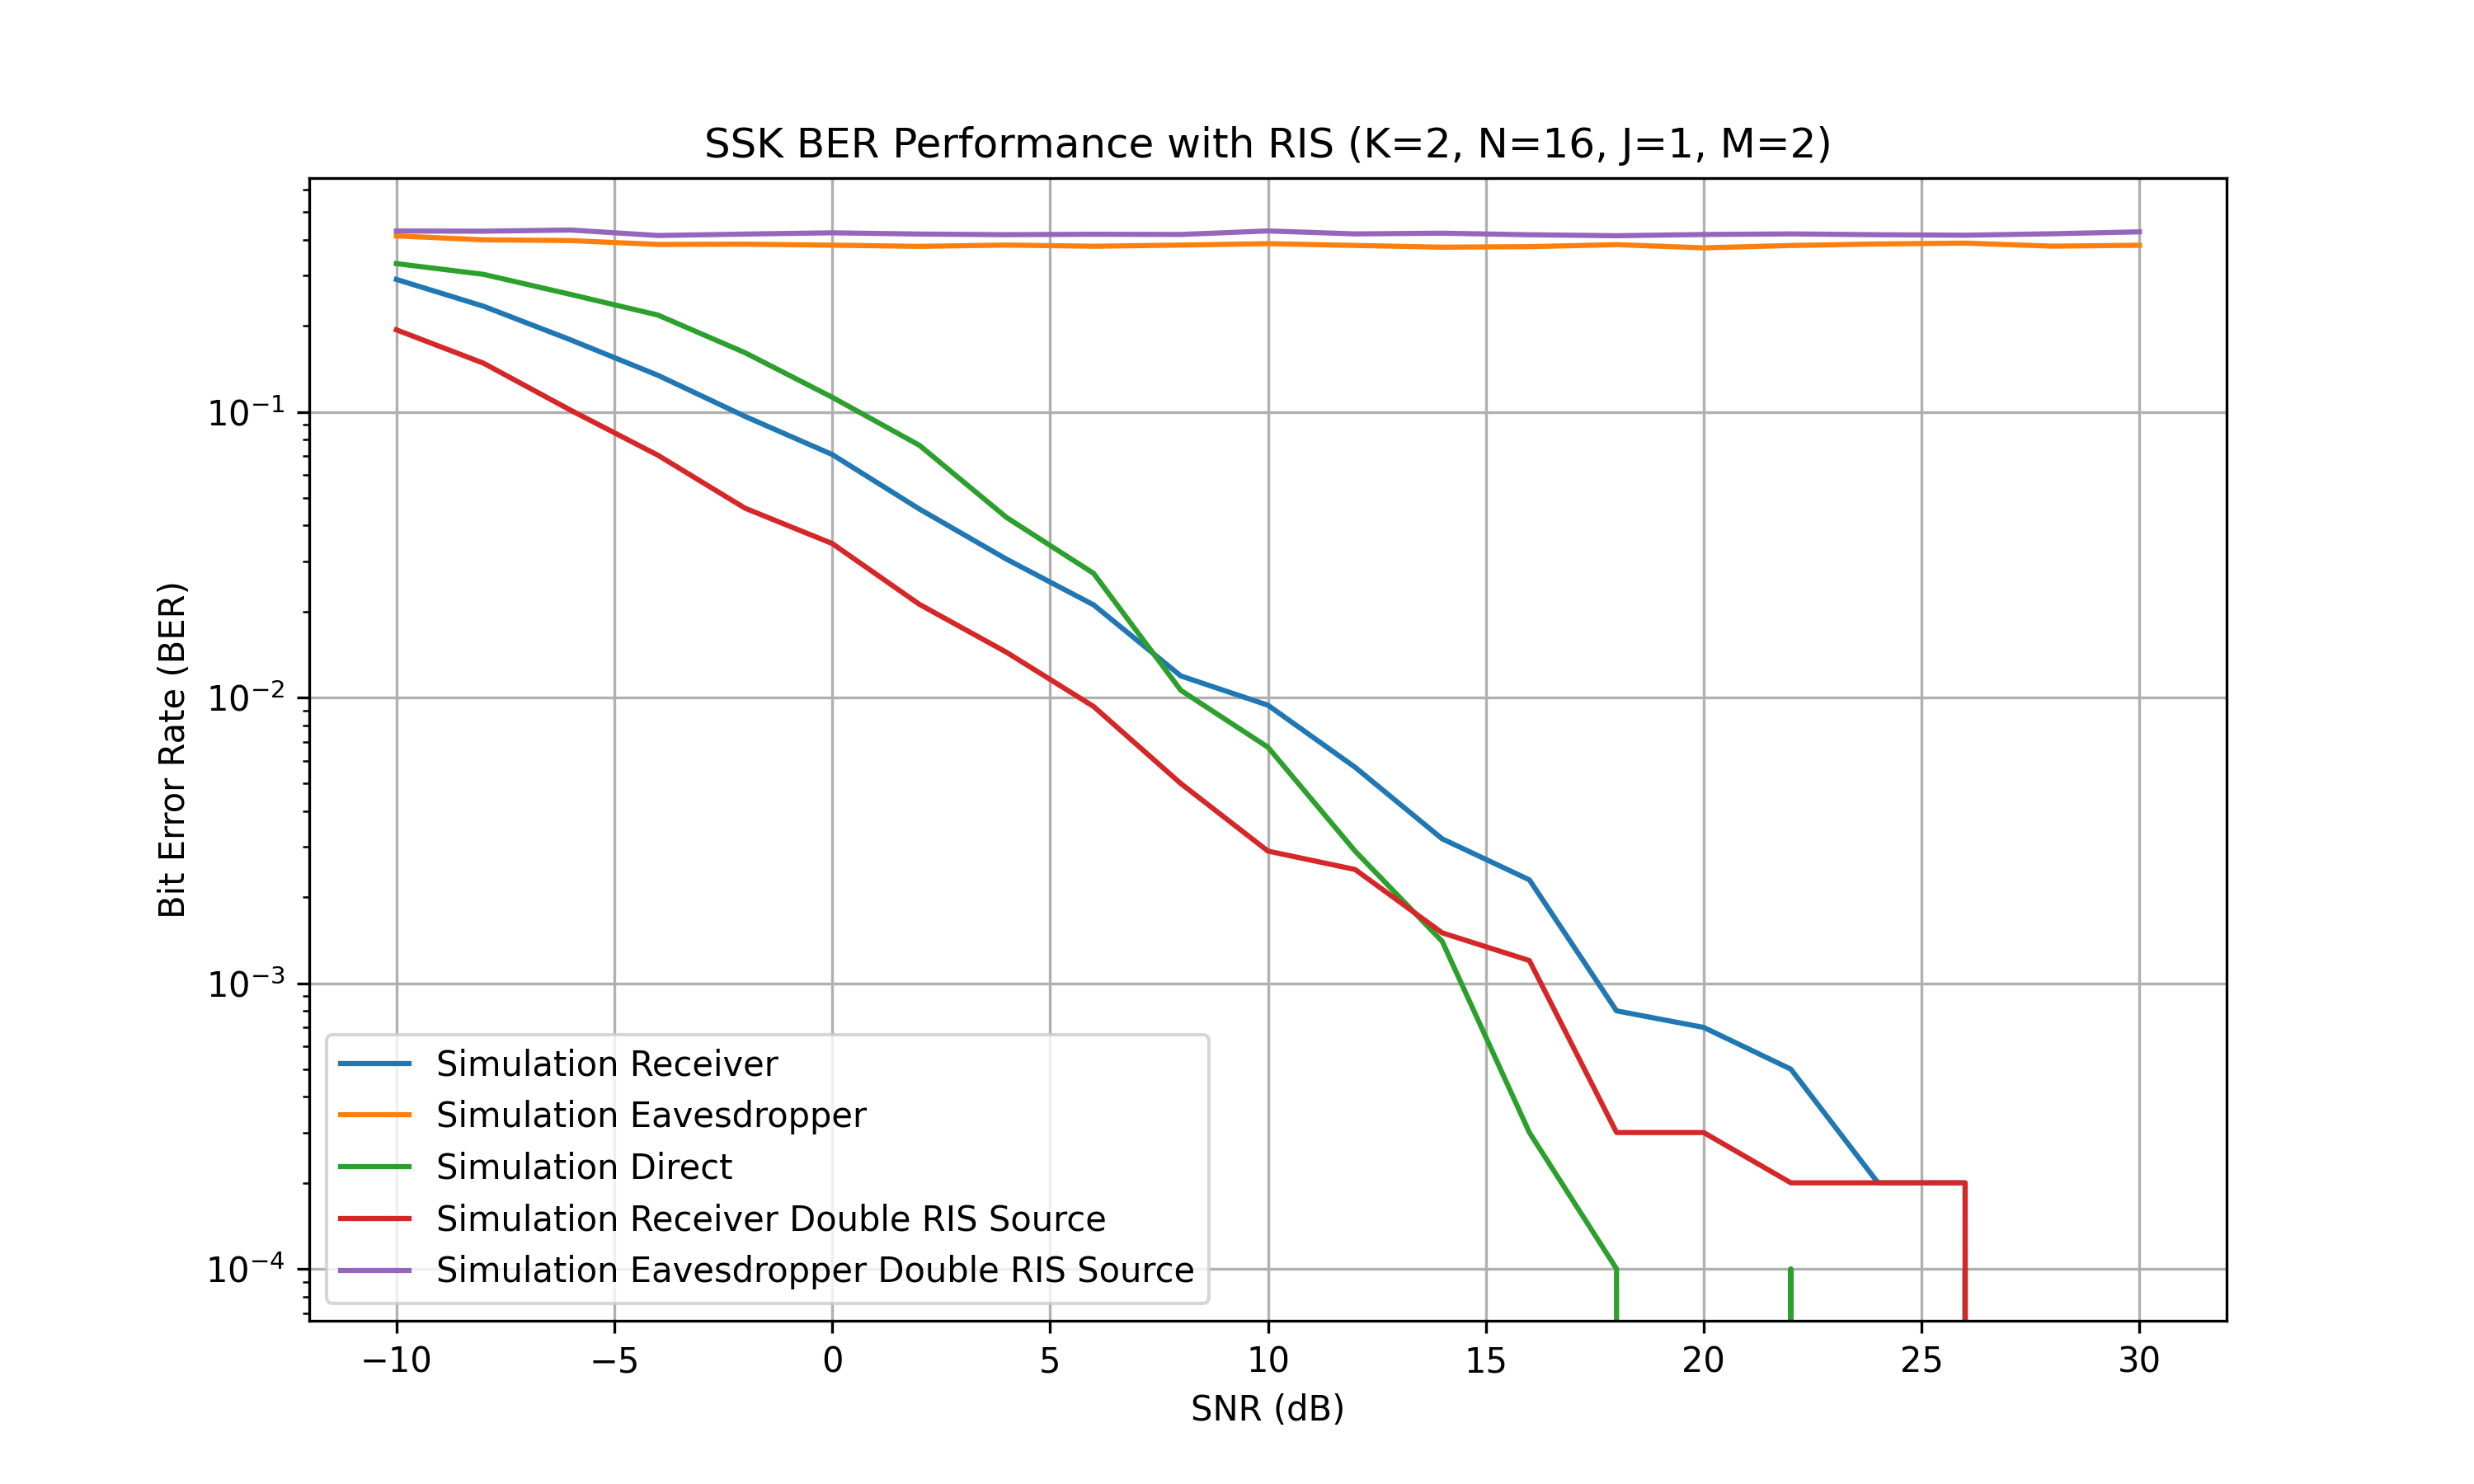
\includegraphics[width=\linewidth]{imgs/ber-simulations/SSK BER Performance with RIS (K=2, N=16, J=1, M=2).png}
  \caption{SSK BER Performance with RIS (K=2, N=16, J=1, M=2)}
  \label{fig:simulation_j1_m2}
\end{figure}

With multiple RIS in series, the eavesdropper get a worse signal because of the double interference of the 2 RIS.
\textbf{(TODO: Why the receiver is getting a better signal? Should it not be worse? Check normalization of the signal)}

\begin{figure}[H]
  \centering
  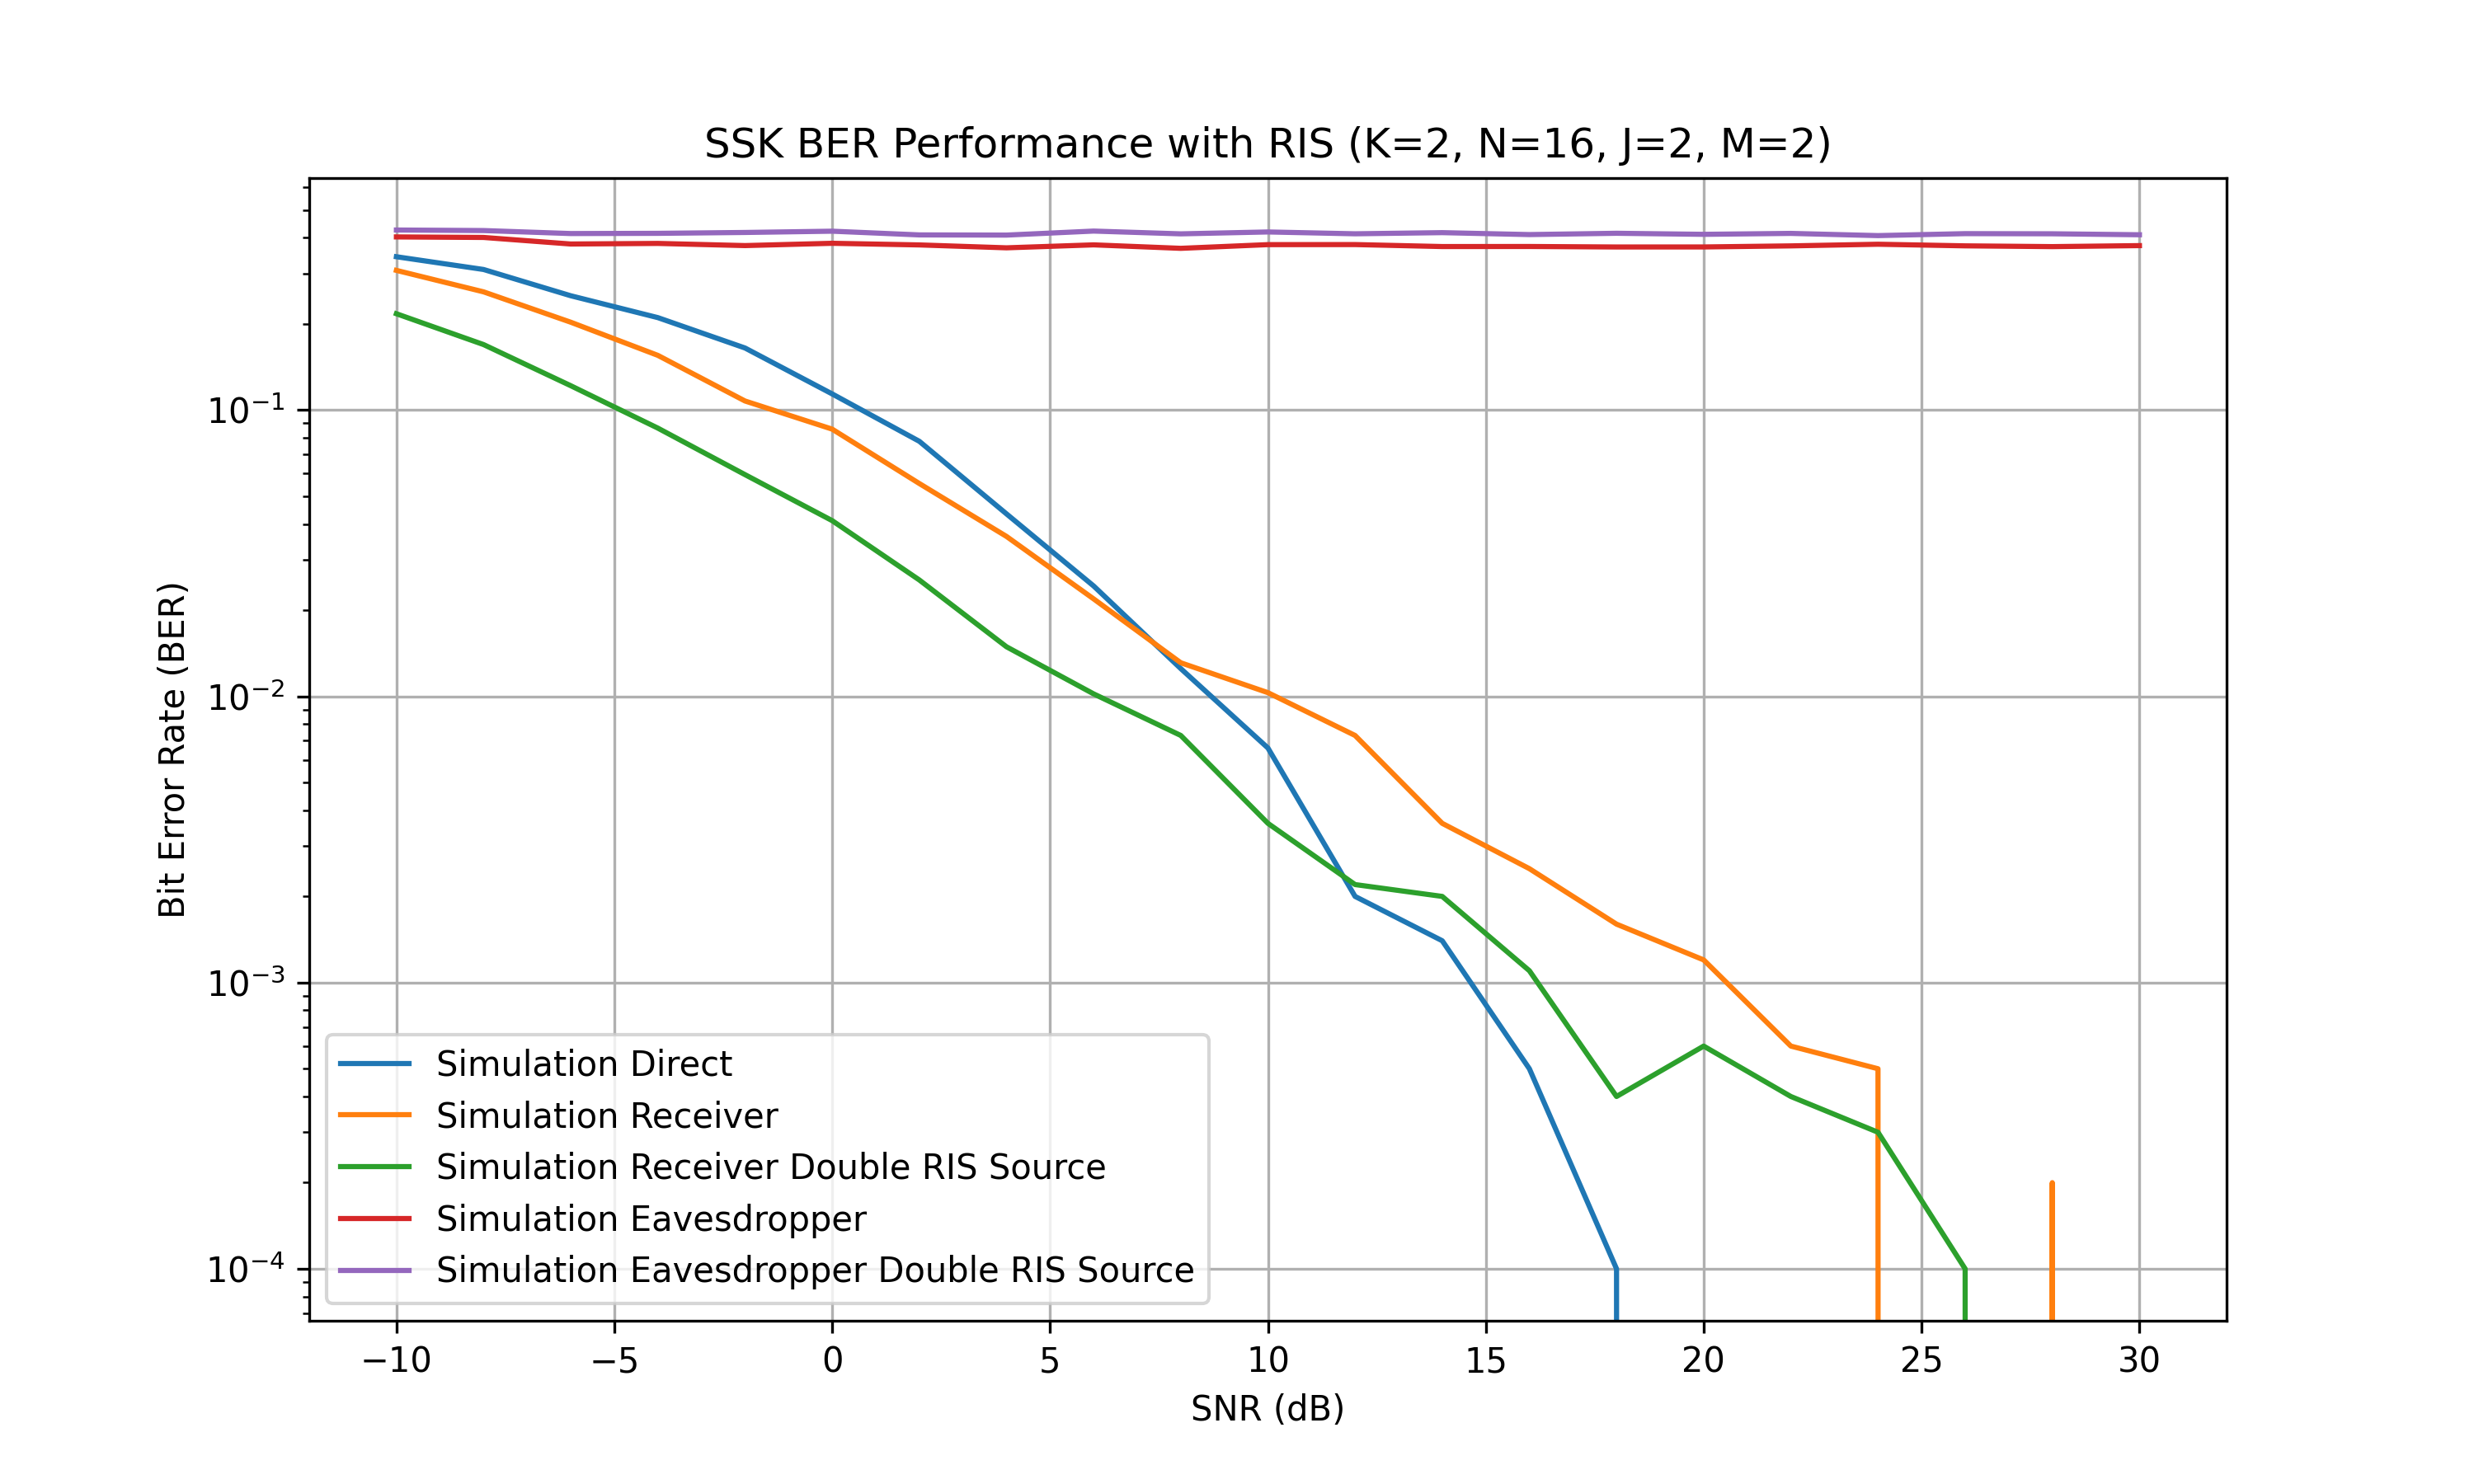
\includegraphics[width=\linewidth]{imgs/ber-simulations/SSK BER Performance with RIS (K=2, N=16, J=2, M=2).png}
  \caption{SSK BER Performance with RIS (K=2, N=16, J=2, M=2)}
  \label{fig:simulation_j2_m2}
\end{figure}

Combining all together, our properties still hold strong.
\newpage
\section{Appendix}

\subsection{Space Shift Keying Modulation}
Space Shift Keying (SSK) Modulation \cite{5165332} is a technique where \textit{antenna indices are used as the only means to relay information}. Given $K$ the number of antenna of the actors in the system, we can send $log_2(K)$ bits by mapping each combination of bits to a specific antenna.
\footnote{This may seem rather unoptimized, as we use only one antenna instead of combinations of them. To see a more general approach, the authors also wrote the paper \cite{4699782}, where they discuss a more general approach.}

\begin{figure}[H]
  \centering
  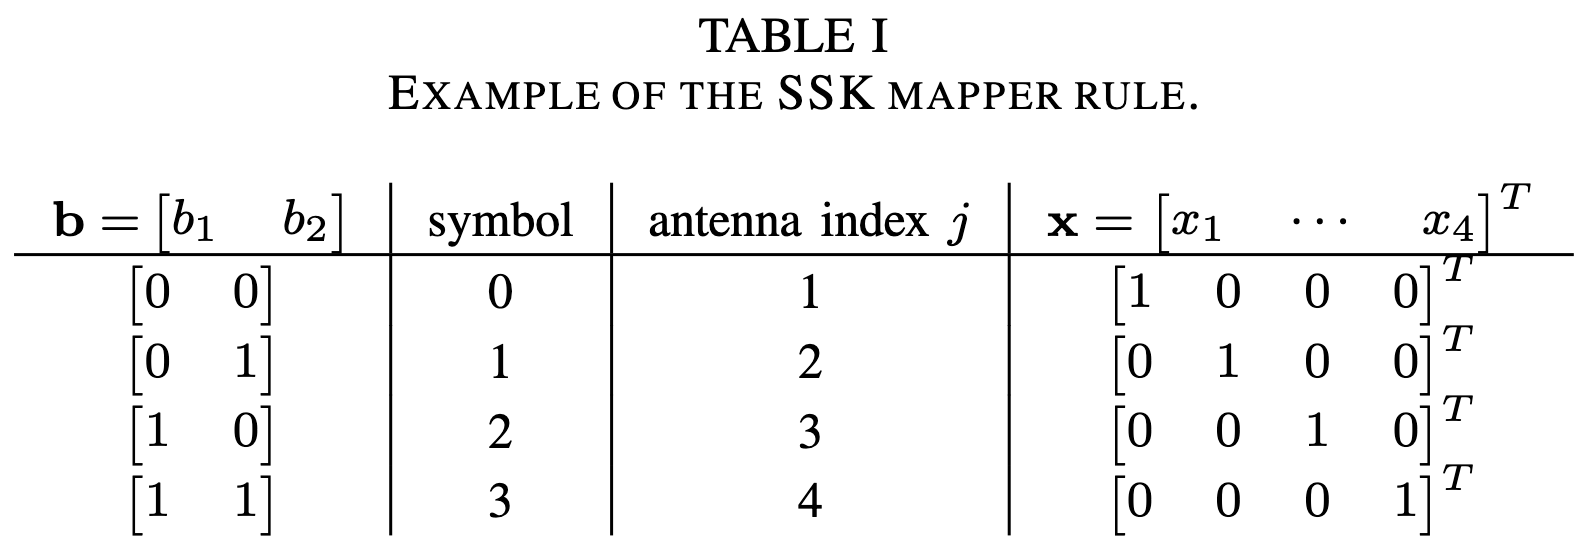
\includegraphics[width=\linewidth]{imgs/ssk_conversion_table.png}
  \caption{SSK conversion table}
  \label{fig:ssk_conversion_table}
\end{figure}

\subsubsection{Direct Detection}
Given a channel gain matrix $B \in \C^{NxN}$ and the input vector $x$ with only one element equal to $1$, the signal received is $y = Bx + \sigma^2$. To understand the antenna index which sent the message, we need to find the column $b_j$ which is most similar to $y$.

\begin{equation}
  j = arg\ max_j\ p_y (y | x_j, B) = arg\ min_j\ || y - b_j ||^2
\end{equation}

\subsubsection{Diagonalized Reflection Detection}
Following \cite{9328149}, for a reflected signal we have $y = GPHx + \sigma^2$. Given that $GPH$ is a diagonal matrix and $x$ has only one element equal to $1$, the resulting vector $GPHx$ will still be a vector with only one element non zero. Adding noise, to find the antenna index we search for the biggest value in the vector.

\begin{equation}
  j = arg\ max_j\ y_j
\end{equation}

\subsection{Cascaded Channel Estimation}
To understand how the actors (and in particular the RISs controller) estimate the channel gain between them, we redirect to the paper \textit{Cascaded Channel Estimation for Large Intelligent Metasurface Assisted Massive MIMO} \cite{8879620}. While we will not summarize the content here, we will still give a general idea of how to use the algorithm in the paper to estimate $G$ and $H$.
\begin{itemize}
  \item The transmitter comunicates to the RIS controller a setup message $x'$ that it will send to the receiver;
  \item The RIS will set a random $P'$; \footnote{As discussed before, in case of multiple RIS in series we set all of them randomly. Later, we setup just the last $P_M$ correctly based on $G'$ and $H$ estimations.}
  \item The receiver gets a signal $y'$ (which will mean nothing), and sends it back to the RIS controller;
  \item Based on $x', y', P'$ the RIS controller estimates $G, H$ and correctly setup $P$;
  \item The transmitter sends $x$, and the receiver gets $y$ which can correctly convert back;
  \item If transmitter and receiver are moving, the procedure will start all over. Otherwise, $G$ and $H$ remain the same, and the RIS controller can just create a new $P$ for the next messages.
\end{itemize}

\bibliographystyle{IEEEtran}
\bibliography{references.bib}

\end{document}



